\documentclass[conference]{IEEEtran}
\usepackage{times}

% numbers option provides compact numerical references in the text. 
\usepackage[numbers]{natbib}
\usepackage{multicol}
\usepackage[bookmarks=true]{hyperref}


\usepackage{amsfonts}                                                           
\usepackage{amsmath}                                                            
\usepackage{amssymb}                                                            
\usepackage{graphicx}                                                           
\usepackage{graphics}                                                           
\usepackage{epsfig}                                                             
\usepackage{mathptmx}                                                           
\usepackage{url}                                                                
\usepackage[l]{floatflt}                                                        
\usepackage{rotating}                                                           
\usepackage{subfigure}                                                          
\usepackage{multicol}                                                           
\usepackage{algorithm}                                                          
\usepackage{algorithmic}                                                        
\usepackage{verbatim}                                                           
\usepackage{listings}                                                           
\usepackage{chngpage} 
\usepackage{bbm}


\DeclareMathAlphabet{\mathcal}{OMS}{cmsy}{m}{n}

\renewcommand{\algorithmicrequire}{\textbf{Input:}}
\renewcommand{\algorithmicensure}{\textbf{Output:}}

\long\def\commentl#1{{\bf **Shih-Yun: #1**}}
\long\def\commentp#1{{\bf **Peter: #1**}}

\begin{document}

%\title{Towards Modeling Real-world Human-robot Interaction that Prevents Overfitting}
\title{Iterative Human-Aware Mobile Robot Navigation}


\author{
    \authorblockN{Shih-Yun Lo, Benito Fernandez, and Peter Stone}
    \authorblockA{
        University of Texas at Austin\\
        {\tt \{yunl;pstone\}@cs.utexas.edu;benito@utexas.edu}
    }
}


\maketitle

\begin{abstract}
Mobile robot navigation in human populated environments has been
widely studied in the past two decades. Significant improvements in
this technology suggest a promising future for introducing mobile
service robots in human workspaces that help with daily
activities. State-of-the-art approaches have shown real-world
deployments of robots that can safely navigate through dense
crowds~\cite{trautman2015robot, pfeiffer2016predicting}. Still, most
robots lack the ability to navigate in a human-friendly manner, which
requires the ability to identify human intentions in situations with
high risk of collision, and to avoid such collisions
“legibly”~\cite{dragan2013legibility}. Most studies to date do not
take human-robot interaction into consideration, resulting in
unexpected human behaviors during deployment, and complicates
planning.  In particular, real-world deployment requires
distinguishing humans who are trying to pass the robot from those who
intentionally block the robot during navigation.  To this end, we
model the planning of pedestrians who are trying to pass the robot as
solving a constrained optimization problem, arriving at their
destination as quickly as possible, while remaining sufficiently far
away from the robot so as not to risk colliding.  People that deviate
from an expected plan can be considered to be interacting directly
with (e.g.\ blocking) the robot.  Preliminary results show that within
this framework, people's paths for passing the robot depend heavily on
the robot's behavior policy, necessitating an incremental training
paradigm that generated expected paths that react to the robot's
current policy, and vice versa.

\end{abstract}

\IEEEpeerreviewmaketitle

%%%%%%%%%%%%%%%%%%%%%%%%%%%%%%%%%%%%%%%%%%%%%%%%%%%%%%%%%%%
%%%%%%%%%%%%%%%%%%%%%%%%%%%%%%%%%%%%%%%%%%%%%%%%%%%%%%%%%%%
%%%%%%%%%%%%%%%%%%%%%%%%%%%%%%%%%%%%%%%%%%%%%%%%%%%%%%%%%%%

\section{Introduction}
\vspace{-0.3em}
\label{sec:intro}
\noindent
% [mobile robot navigation advances in dynamic environment]
%In robotics, recent advances have allowed long-term autonomy for indoor mobile 
%robot navigation, which has raised interest in the development of service 
%robots that provide assistance to humans during daily activities. To achieve 
%this objective, the robots need to be able to navigate smoothly among pedestrians, while 
%not interfering with their ongoing activities. 
%%This problem involves 
%%modeling well the dynamics in human-robot interaction, where individuals have 
%%independent goals to reach and potential collisions need to be avoided. 

% [human robot interaction scenarios]
Consider a robot navigating in a busy atrium with people walking
towards different destinations. 
%Both the robot and the pedestrians
%generally have limited sensing of nearby agents.  
%In general, it is not enough for the robot to
%reactively avoid imminent collisions. 
To navigate robustly, the robot must both predict the motions of approaching pedestrians, and plan its own motions so as not to collide with their predicted paths.
When doing so, it is not sufficient to consider the paths of pedestrians as 
fixed.  Rather, the robot needs to recognize that its own behaviors can 
impact those of the pedestrians. That is, the robot and pedestrians are all a 
part of a tightly coupled multiagent navigation 
problem. 



%However, when predicting into
%the future, collision avoidance algorithms often fail to find a path
%in densely crowded environments, sometimes referred to as the
%"freezing robot problem"~\cite{trautman2010unfreezing}. For example,
%in human pedestrian navigation, it is commonly seen for agents to walk
%in front of one another to maximize their own travel efficiency,
%assuming other pedestrians are aware of the workspace occlusion and
%respond safely. Can the robot act the same way, while optimizing the
%joint efficiency of both agents?

% [state of the art robot navigation in crowd]
%To plan efficiently in dense crowds at the same time maintaining 
%human-friendliness and safety, it is crucial to have good models of human 
%responses to the robot's maneuvers. 
Many approaches have been proposed in the 
past decade to simulate human pedestrian dynamics in crowds~\cite{helbing1995social,lamarche2004crowd, 
  %treuille2006continuum, %paris2007pedestrian, 
karamouzas2009predictive}, and have provided insights into human collision avoidance behaviors.
%Accordingly, robot planning in crowds has shown efficient performance in simulation
%These models have been used for look ahead planning.
However, 
%to consider a \emph{robot} planning in crowds, 
behaviors observed among human pedestrians may not fully 
repreent their dynamics when interacting with a \emph{robot}. 
In particular, when deploying a robot in the real world using state-of-the art approaches, there has been a 
large gap between the predicted pedestrian motion and observed trajectories~\cite{trautman2015robot,pfeiffer2016predicting}. 
None of the robot planning work in the literature has been based on realistic human-robot dynamics,
 which has lead to inefficient and/or unsafe robot behaviors.

%%to eliminate the gap between human-robot interaction modeling and real-world deployment
In this paper, we propose to solve the \emph{robot navigation 
in crowds} problem by taking into account the pedestrian's reactions to the 
\emph{robot's} motions, to ultimately optimize the expected joint efficiency 
of the robot's and the pedestrian's motions. We start with the study of human 
collision avoidance behaviors subject to robot's maneuvers, and pay close 
attention to scenarios with crossing paths, as illustrated in Fig.~\ref{fig1}.

In such situations with anticipated workspace occlusion,
%\commentp{I don't know what future workspace occlusion means}
pedestrian paths fall into two homotopy classes: either passing in front of the 
robot (or other pedestrian), or behind it. Such behaviors capture the dynamics of 
goal-focused people in a workspace occlusion scenario, which can therefore 
be used to distinguish motions that are directly interacting with the robot, such as 
intentional blocking.


%\commentp{That last sentence is too complex.  What are "social interaction preferences"?  Is intentional blocking a preference or a behavior?}


%The robot can 
%then optimize the joint efficiency by avoiding responsively to their 
%preferences, legibly, such that the pedestrian 
%is clear about the robot's intention. Our model then predicts cooperative behavior from rational pedestrians; non-cooperative behavior, such as intentional blocking, can therefore be distinguished if the pedestrian does not follow any expected patterns.

%Towards the deployment of a service robot in real world, the robust guarantee of safety during human robot interaction is important. Still, state-of-the-art modeling of this joint dynamics has limited capability when pedestrians engage in behaviors not presented in the training data. With complex model and unbalanced training data, the prediction model is under high risk of overfitting.

From gathering real-world human-robot interaction data, we 
observed that different people have very different strategies over path 
decisions. We therefore propose a psychological model of their decision making 
process to capture factors that potentially influence those different avoidance 
strategies. Such a model helps us identify a particular person's strategy as it 
approaches the robot, to further select features to train a predictive model 
over path decisions.
 

We also observed that changing the robot behavior
can lead to different pedestrian behavior.  We therefore
propose an iterative learning process by which the robot acts
according to its current learned predictive pedestrian motion model
to gather revised data to incorporate within a new model.  This
process is designed to help ensure consistency between the robot's
prediction of pedestrians' trajectories and their true trajectories in
the presence of the mobile robots.

%With this process, we aim to achieve robot planning in 
%crowds that not only follows the inherent interaction patterns in human 
%pedestrians, but also counts in the noisy interaction where people intentional 
%block the robot.

%% to deal with human intentions for trajectory prediction
%To achieve smooth robot maneuvering in human crowds, it is essential to 
%systematically identify whether the person is focused on 
%reaching their goal (conducting natural navigating behaviors), or may be 
%distracted by the presence of robot (conducting unnatural navigating 
%behaviors, such as blocking). To model this problem, we propose to first 
%enable prediction of human traversal behaviors when encountering potential 
%collisions, shown in Fig.~\ref{fig1}. 

%We consider the scenario, illustrated in Figure~\ref{fig1}, in which a
%person may have one of two possible intentions: slowing down to pass
%behind the robot or speeding up to pass in front of it.  To navigate
%safely towards its goal, the robot must predict the pedestrian's
%intention, and possibly plan to influence it.  In addition, the robot
%must consider the possibility that the person will intentially
%interact with the robot (e.g.\ to block its path and "play" with it).


\begin{figure}[t]
  \begin{center}
  \hspace*{-1em}
  \subfigure[0.45\columnwidth][] {
    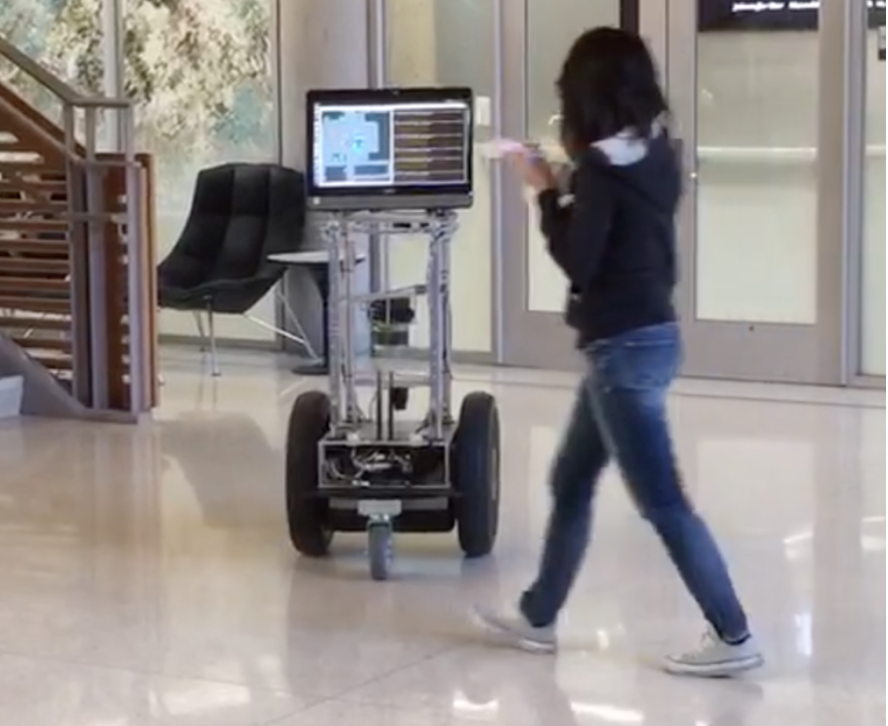
\includegraphics[width=0.5\columnwidth]{p1.png}
    \label{fig:p1}
  }\hspace*{-0.03em}
  \subfigure[0.45\columnwidth][] {
    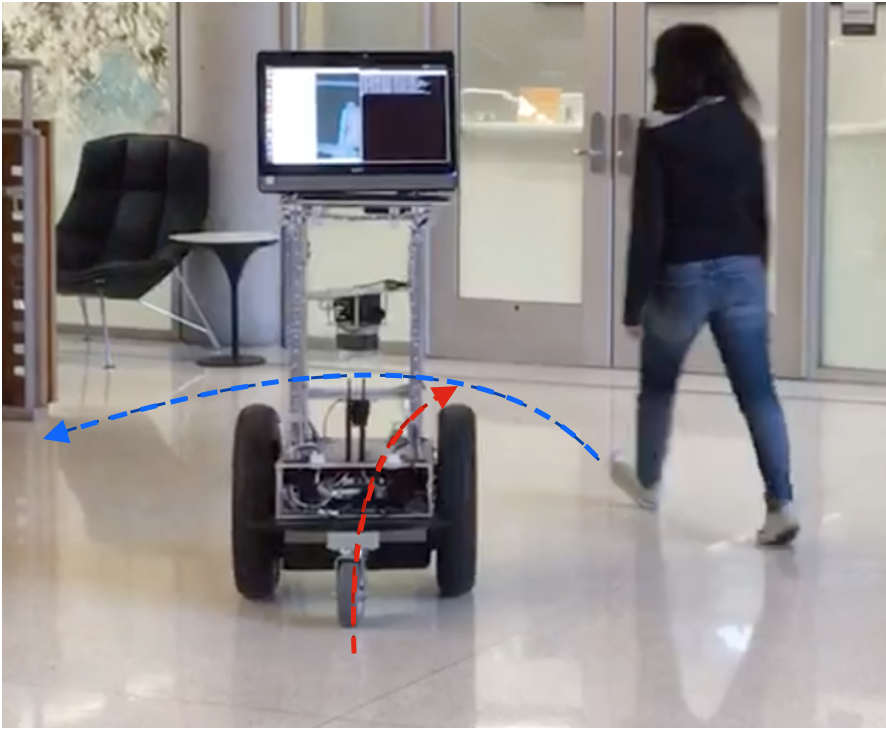
\includegraphics[width=0.5\columnwidth]{p2.png}
    \label{fig:p2}
  }
  \end{center}
  \vspace{-0.85em}
  \caption{The two pictures illustrate the common patterns of human 
    pedestrians passing the other agent (here the robot) to avoid a potential 
    collision (with the robot 
    moving towards the door, the pedestrian moving to the stair case at the left): {\bf (a)} to 
    decelerate and wait for the robot passing in front, 
    {\bf (b)} to accelerate and pass in front of the robot. %Two styles of 
    %traversal trade off between total path lengths and end speeds. 
    While 
    slowing down to wait results in shorter paths, speeding up to pass in 
    front is also commonly observed when people navigate in crowds. 
    }  
  \vspace{-1em}
\label{fig1}
\end{figure}


%When the robot performs 
%``legibly''~\cite{dragan2013legibility} in those 
%situations, non-cooperative behaviors (intentional blocking) can be identified if not 
%classified into any type of traversal. 

 %we also propose to model the interactive dynamics based on local 
%observations, which helps the applicability of the approach in varied 
%environments. It is a contrained optimization problem on temporal collision 
%including its safety margins. The prediction process then falls in first deciding 
%which way the agent is prone to take, and how it would adapt its dynamics during 
%traversal. Accordingly, the controller looks ahead and optimizes the joint 
%efficiency subjected to the estimate of human traversal preferences.

%To this end, we model goal-oriented pedestrians as solving a constrained path optimization 
%problem, which maintains safe distances from other agents while trying to reach
%their destination as quickly as possible. 
%This approach provides us the 
%capability to predict which path the 
%pedestrian is prone to take to avoid, at what speed pattern. 
%**************FIX REST OF THIS PARAGRAPH

% local sensing, local representation (no global goal)
% the limited predicting capability when people engage in behaviors not present in the training data
%When navigating in a crowded environment, people observe other agents' behaviors, and act accordingly. With different dynamics observed, people conduct different motion patterns. The same situation applies to human robot interaction as well. If the pedestrians observe aggressive behaviors during robot navigation, they may perform conservatively by staying away from the robot to avoid collision; if the robot appears to be respond safely to disturbances in the environment, people may trust the robot more and interact with it more closely. 
%To solve this problem, we acknowledge that different pedestrian behaviors are excited under different robot maneuver policies. The learnt pedestrian dynamics may only capture partial interactive behaviors with the robot given its conducted policy. For example, if the robot navigates in the crowd with conservative avoiding behaviors, the learnt interaction would be limited as treated as a static obstacle; on the other hand, aggressive robot navigation may result in pedestrian avoiding behaviors where limited interaction is experienced. 

% introduce this work that does not overfit



\vspace{-0.2em}
\section{Related Work}
\label{sec:related}
\vspace{-0.4em}
% recent advance in crowd navigation modeling
% a) physics-based modeling of pedestrian spacing 
% b) inverse optimal planning techniques
The earliest attempt to model pedestrian behaviors was through a physics-based 
modeling approach, in which the spacing between pedestrians follows a 
potential field to generate collision-safe 
interactions~\cite{helbing1995social}. Following this work, explicit models 
for local collision avoidance were widely studied, to model the subtle 
adaptive personal-spacing behaviors in pedestrian 
interactions~\cite{papadakis2014adaptive}. Meanwhile, another community 
makes use of inverse optimal planning 
techniques~\cite{ziebart2009planning,henry2010learning,vasquez2014inverse} to 
model pedestrian dynamics by learning their policies assuming global observations and 
rational behaviors.
% a,b ignore the interactive dynamics in which one player's action affects the other's 
% c) joint decision making process
While the above approaches have been shown to predict pedestrian motions 
offline or in simulation, an issue arose with the Markov Decision 
Process assumption when the methods were deployed on a robot to navigate in the real world:
the real-time dynamics of pedestrians are also dependent on the robot's 
actions. 
%While the pedestrians treat the robot as an agent, they plan 
%accordingly to robot's motion. 

In this regard, a multi-player game setting including both human and robot actions into the joint state space was proposed and evaluated on a mobile robot in a fully-observed environment~\cite{trautman2010unfreezing}. This game setting has also shown significant results in autonomous cars through the consideration of human actions into their model to achieve communicative robot behaviors~\cite{sadigh2016planning}.
% d) prediction using offline training data does not always work: data may be from rational agents. Further, interactive data may only go from a small portion of state space, excited by pre-defined robot behavior 
Still, all of the above work are built from data collected by observing human-human 
interaction, which has degraded planning performance while encountering unmodeled 
human-robot interactions during real-world 
deployment~\cite{trautman2015robot, pfeiffer2016predicting}. To achieve 
cooperative interaction with humans and robots sharing a workspace, it is 
an essential capability for the robot to identify people's 
intentions, and then plan responsively to their actions. We propose to achieve 
better human-robot interaction in crowds by learning a predictive model 
iteratively through online interaction, and propose a predictive model 
that generates plans to avoid dynamic obstacles based on personal walking features. 
\vspace{-0.1em}
\section{Methodology}
\vspace{-0.1em}
The following is a receding-horizon control formulation of the constrained 
optimization problem characterizing the pedestrian's motion. The control 
$u \in \mathbbm{R}^2$ 
%\commentp{"takes in" is awkward.  Can we just say $u \in \mathbbm{R}^2$?}
is defined as the acceleration of the pedestrian, with 
position $x^p \in \mathbbm{R}^2$ and velocity $v^p \in \mathbbm{R}^2$. We  
consider
%\commentp{I don't know what "take in" means here either.  Do you mean "We assume a discrete state space"?}
discrete system dynamics in continuous state space, so $x_{t+1}^p = v_t^p + v_t^p dt$.
%\commentp{isn't that a continuous, not discrete forumulation?}
Similarly, we denote the ''opponent's'' position $x^o$ and velocity $v^o$. We assume that, 
people plan with a receding-horizon strategy, namely to plan ahead for a fixed 
horizon from time $t$ to $t+N$, act according to $u_t$, and start over on the 
next time step $t+1$:

%constraints on 
%the temporal collisions with 
%(adaptive) safety margins $r^{saf}$. \commentp{Is that a sentence fragment left over from something?  There needs to be some lead in to the equations such as what I suggested below.}
%More specifically, we model the pedestrian 
%planning with a receding-horizon strategy, adopting a similar cost formulation with Model 
%Predictive Control, over $N$ time steps.
%\commentp{Write something like:  The following is an LP formulation of the contrained optimization problem modeling the pedestrian's motion.  (and you haven't defined x, u, or even the velocities as a funcntion of time - the t subscripts.  Can't $r^{rel}$ be defeined in terms of the x's?}
%$r^{rel} = (x^p-x^o)^T(x^p-x^o)$,
%where $x^p, x^o$ are the positions of the two agents and the location where an expected collision will happen 
\begin{equation}~\label{eq:receding_control}
  \begin{aligned}
    &min_{u_n \dots u_N} \Sigma^N_{t=n} \small{C_{length,t} + C_{energy,t} + C_{social,t}} + C_{to-go,N}\\
    & (r^{rel}_t)^2 > (r^{{saf})^2}\\
    & v^p_t < v_{max}\\
    & x^p_{t+1} = x^p_t + v^p_t \scriptsize{d}t\\
    & x^o_{t+1} = x^o_t + v^o_t \scriptsize{d}t\\
    & v^p_t = v^p_0, t \leq n\\
    & v^o_t = v^o_0\\
    & v^p_{t+1} = v^p_t + u_t \scriptsize{d}t, t>n.
 \end{aligned}
\end{equation}
We assume that the pedestrian has some rough estimate of 
his/her own velocity $v^p$, the opponent's velocity $v^o$, both agents' 
desired(initial) velocity $v^p_0, v^o_0$, and their relative distance 
$r^{rel} = (x^p-x^o)^T(x^p-x^o))$.
The inequality constraints are posed on the pedestrian's (adaptive) safety margin 
$r^{saf}$ between two 
agents, and the pedestrian velocity upper-bound $v_{max}$. 
The equality constraints are posed on the 
dynamics of both agents and their initial velocities 
$v^p_0, v^o_0$, which the robot can estimate based on past 
observations through filtering techniques. 

The control input $u$ is not bounded but 
penalized in $C_{energy}$ for acceleration/velocity variation of the trajectory. 
$C_{length}$ and $C_{to-go}$ penalize path length and a heuristic cost-to-go. 
Following a standard quadratic formulation in optimal control, we have: $C_{energy,t}=u_t^TRu_t$, 
$C_{length,t}=\delta_t^TQ\delta_t$, $\delta_t = x_{t+1}-x_t$, 
$C_{N,to-go} = (x_N-x^G)^TP_N(x_N-x^G)$, where $x^G$ is the (sub)goal 
position of the pedestrian. $P_N$ can be solved through dynamic programming:
$P_N = Q + K_N^TRK_N + (A+BK_N)^TP_N(A+BK_N)$, 
$K_N = -(R+B^TP_{N-1}B)^{-1}B^TP_{N-1}A$, considering a linear system dynamics
$s^p_{t+1}= As^p_t+Bu_t$, here $s^p = [x^p,$ $v^p]$. $Q$ and $R$ are positive 
semi-definite matrices. Other forms of cost-to-go can also be adopted, such as 
naive distance estimate (considering only distance-to-go), or social 
cost-to-go estimate (such as considering end-pose distance with a large group 
of static people).
%\commentp{What's a social cost-to-go estimate?}
%`(for example, to incorporate 
%potential road-blocking by a group of static pedestrians nearby).  
%$C_{social}$ may take in the form considered in social 
%proximity model~\cite{kruse2012legible}, social force 
%model~\cite{helbing1995social}$\ldots$ etc, to maintain the social 
%friendliness in crowd navigation. 

$C_{social}$ represents the pedestrian's social interaction tendencies when 
navigating in a crowd. More specifically, based on
studies of robot legible motion in 
navigation~\cite{kruse2012legible,lichtenthaler2012influence} and human 
spacing/dynamics in crowds~\cite{helbing1995social,hall1966hidden}, we design 
the social cost function $C_{social}$ to include \textit{visibility}, and \textit{comfort}, 
to explain human crossing path selection:
\begin{equation}~\label{eq:social_cost}
  \begin{aligned}
    C_{social} &= \omega^T f(x), \\
    f(x) &= [C_{vis}, C_{comf}],
  \end{aligned}
\end{equation}
where $\omega$ is a weighting function.
As suggested in ~\cite{kruse2012legible}, when planning for crossing, people 
prefer the traversing path that maintains visibility from the point of view of 
the other agent (i.e. passing in front).
%\commentp{Say visibility of what:  people prefer the traversing path that maintains visibility from the point of view of the other agent (i.e.\ passing in front).}
From the social force formulation~\cite{helbing1995social}, velocity with a 
large component along the other agent's opposite direction 
%velocity \commentp{What is confronting velocity?  Do you mean relative velocity?  Velocity with a large component along the line pointing directly at the other agent?}
causes higher repellent forces.
%(therefore higher cost function gradient). 
%\commentp{repellant forces of whom from what?   What's the cost function gradient?  You're using terms without defining them here again....}
We model this repellent force to be caused from a cost function referred
%\commentp{What is "it"?}
as social discomfort, 
%defined as having high confronting velocity\commentp{Still don't know what that means.} 
which appears when the opponent agent is within the pedestrian's social space:
\begin{equation}
  C_{comf} = (v^p-v^o)^T (v^p) \mathbbm{1}(r^{rel}<r^{soc}).
\end{equation}
This term penalizes crossing behaviors that turn towards the opponent agent. 
%therefore limits the pedestrian from speeding up and crossing from far behind. 
%\commentp{Can we just delete "for crossing" and still have this make sense?}
Along with visibility assessment, the pedestrian who chooses to pass 
behind has an even higher cost to speed up compared with the maneuver to pass 
in front. This contributes to the commonly seen slowing-down behavior in $a^P$, 
which results in the pedestrian staying mostly on the original route, 
%\commentp{I don't know what "are modeled to slow down" means} 
shown in Fig.~\ref{fig:p1}.
%Note that, here we hypothesize a (adaptive) response 
%time $n$ before the person act according to the cost function, which we refer 
%to the psychological tension before reacting to mental 
%decisions~\cite{helbing1995}. With that said, the person may have decided to 
%change path to avoid, but it takes a while for he/she to really take the action.

Note that we build into our model a (adaptive) response 
time $n$ before the person acts according to the cost function, following the notion of
\emph{psychological tension} before reacting to mental 
decisions~\cite{helbing1995social}.  This variable, reflected in 
Eq.~\ref{eq:receding_control} allows us to capture the fact that the person may 
have decided to change paths before he/she actually takes the action.

%%%%%%%%%%%% homotopy class explanation
%The temporal collision constraints
%divides the 2D planning configuration space into two 
%homotopy classes,
%\commentp{is there a way to get the homotopy classes from the equations?  How?  By processing/solving them in some way?}
%which leads to two commonly observed crossing path decisions 
%in a two-player scenario: slowing down and traversing from behind by 
%removing the expected occupation
%\commentp{say who is expecting and who is occupying}
% at the projected intersection
%\commentp{you haven't yet refered to/defined what is the projected intersection.  Is% it in the equations?}
%(passive action, $a^{p}$, as 
%shown in Fig.~\ref{fig:p1}), as well as to speeding up and passing in front by postp%oning 
%the expected intersection (active action, $a^a$ as shown in Fig.~\ref{fig:p2}).

%Note that, from the path planning perspective, there exists another homotopy 
%class symmetric to that of passing in front:  turning towards the 
%opponent agent then speeding up. \commentp{to pass behind it quickly}
%by turning some degrees towards the other agent, 
%This maneuver results in earlier crossing time\commentp{crossing time also wasn't defined.  Is it reflected in thequations?}
%than the other two options, and\commentp{but?} 
%is seldom seen in crowds because of the inconsistency between intention 
%(passive traversal from behind) and motion pattern (active traversal by 
%speeding up). The path length is long and the confronting action raises the 
%risk of breaking in front of the other agent's safety margin. 
%\commentp{I don't understand "breaking in front of the other agent's safety margin".  Breaking down?  Why in front?  Isn't the path behind?}
%\commentp{Do you mean to say that we don't consider this homotopy class?  You don't say that so far...}

%% state space representation, 
% from robot's perspective, with a figure showing desired vel, goal..etc
%\vspace{-.2em}
%\subsection{Human Crossing Decision Hypothesis} 
%To model human path planning behaviors, we either assumes a behavior model 

%we can assign costs to 
%the observed path, and there are different approaches to explain or predict 
%the likelihood of such path based on assumptions on the decision making 
%process~\cite{ratliff2006maximum, ziebart2008maximum}, or cost function 
%formulations~\cite{kruse2012legible}. For example, in 
%\cite{trautman2010unfreezing}, the authors collected data on human 
%navigation in crowds, and proposed the Gaussian 
%process mixture model to predict in real-time the pedestrian paths. 
%Due to the goal-imposed behavior formulation (which highly limits the applicability of 
%their approach in different domains), this model is also used during robot planning. 

%With our constrained optimization setting on human path planning subject to the other agent 
%crossing (shown in Eq.~\ref{eq:receding_control}), from an inverse optimal 
%planning perspective, we can learn the cost function of human traversal 


%The crossing path decisions vary much among different people, 
%which we can 
%explain through Eq.~\ref{eq:receding_control} on the different values of response 
%time $n$, safety margin $r^{saf}$, navigation social preference weighting 
%$\omega$, and possibly the weighting on other cost terms. Those psychological 
%and social preference factors of a person can also vary when the confronting 
%agent is different, for example, a robot rather than a human.

%\commentp{Is this what you mean for the prior paragraph?}
%We find that different people plan different paths even when facing the same situation, 
The crossing path decisions vary much among different people, 
which we can explain through the variables in Eq.~\ref{eq:receding_control}, such as 
$n$ (response time), $r^{saf}$ (safety margin), $\omega$ (social cost 
weighting function)
%\commentp{I don't understand what that means.  And you never actually defined $\omega$ above...}, 
and possibly the weighting on other cost terms in Eq.~\ref{eq:receding_control}
%\commentp{such as?}. 
Those psychological 
and social preference factors of a person can also vary based on the crossing
agent, for example, a robot rather than a human.
%\commentp{You need to decide on a word to describe the other agent and stick with it.  Opponent?  Confronting agent?  Other agent?  Earlier you were using "opponent", and that's what the notation suggests.  But maybe "other agent" or "crossing agent" is better.}

As suggested in ~\cite{hansen2009adaptive},
people have different degrees of interest/comfort in interacting with a robot, which 
can affect their maneuvers during human-robot crossing. For 
example, in human crowd dynamics simulation, the safety margin is considered 
merely a function of crowd density and walking speed~\cite{helbing1995social},
whereas in real-world robot deployments, we observe that this variable can vary a lot from person to person.
%but vary a lot from person to person around a robot, as observed during robot 
%real-world deployment. 
%\commentp{I edited that sentence.  Is it still correct?}

To predict human-robot crossing behaviors, it is therefore insufficient to learn
one set of parameters from one large set of interaction data across many people. 
%the lump-sum interaction data in the predictive mode
%\commentp{I edited the above because I didn't understand "in the predictive mode"}
%\commentp{I'm not able to follow the point of the rest of this paragraph.}
Further, the changes in the pedestrian's dynamic behavior can be sudden when he/she react 
to the crossing decisions (considering 
sudden pedestrian dynamics changes at time $n$), and the 
trajectories associated with different crossing decisions can have largely 
different dynamical performance. Therefore, false 
prediction can much deteriorate the joint path efficiency, and possibly the 
safety criteria. 
%Same is true for the response time. In 
%Eq.~\ref{eq:receding_control}, we consider the agent to plan by looking ahead 
%$N$ time steps, and start reacting from the $n_{th}$. Those values may also largely 
%vary based on their perceptions of the robot, such as: is the robot safe?  

%Coming back to Eq.~\ref{eq:social_cost}, it suggests that people may have 
%very different values of $\omega$, resulting in different path planning 
%strategies in collision-potential scenarios, which adds up the complexity of the 
%algorithm to incorporate personal differences in $\omega$: how do we 
%distinguish it from the stochacity in human decision making process? 

%And the inverse optimal planning practice would be to optimize a fixed 
%$\omega$ that maximizes the likelihood function $P$ based on observed 
%trajectories $\xi$,
%\begin{equation}
%  max_{\omega} P(\xi|\omega).
%\end{equation}


%Coming back to the application of pedestrian motion prediction and the 
%robot planning accordingly, if one were to extract the motion features of a 
%person given past observation, to predict the weights on the cost function for 
%social preferences, the overall cost function formulation would be to learn 
%a functional mapping $w$ as a function of the dynamic features of the person. 

%One solution to maintain the tractability of the model, especially under 
%limited data from real-world experience, is to enforce sparsity if $\omega$ is 
%presented as a functional mapping. This approach can be understood as to limit 
%the variety of traversal preferences.

However, to identify all those variables seems computationally intractable 
from a model training perspective. For example, for inverse optimal planning, 
the algorithm seeks to find a fixed $\omega$ in 
Eq.~\ref{eq:social_cost} that maximizes the likelihood function $P$ of 
observed trajectories $\xi$,
\begin{equation}
  max_{\omega} P(\xi|\omega),
\end{equation}
and trajectories representing different values of $\omega$ need to first be 
classified, or the algorithm will not converge. 

Still, to plan in the crowd, humans do a successful job without accurate 
prediction, and false prediction is even commonly observed without necessary 
safety harm. For example, with a direct confronting agent in the front walking 
towards you, people sometimes avoid to the same side at the same time (or 
within close time). What seems to matter is then just \textit{which way} 
to go instead of the entire trajectory prediction. 

We therefore propose to seek for a much simpler predictor over pedestrian path 
crossing decision manifold: to pass from the front ($a^P$) or behind($a^A$), 
through logistic regression,
\begin{equation}
p(a=a^P|\xi^p_t, s_t) \sim \frac{1}{1+e^{w^Tf(\xi^p_t, s_t)}}.
\end{equation}
Here, $s_t = [x^p_t$, $v^p_t$, $x^o_t$, $v^o_t]$ is the state of the overall 
system, included to characterize the crossing scenario;  $\xi^p_t$ is the past 
trajectory of the pedestrian at time $t$, included to characterize the 
pedestrian's the dynamic patterns, and $f$ is a feature function.

%%%%crossing function

We propose to iteratively learn this predictive model through robot's real-world 
deployment. Since people are also adaptive about their reaction to a robot, 
new types of behaviors may be observed over time.

\vspace{-.3em}
\subsection{Intention Expression and Opponent Response Hypothesis during Human Crossing}
%% intention indiated behind speed patterns. 
When people decide their path for crossing, the\commentp{whose?  their?} \textit{dynamic patterns} of 
motion, such as speeding up and turning away, indicate the\commentp{whose?  their?} intended path 
decision, which we refer in this paper as the \textit{intention}: the 
intention to actively cross the other agent from the front by speeding up($a^A$), 
or to passively cross from behind by slowing down($a^P$).


%This somehow differs from the 
%definition of legibility as being goal-expressive in 
%~\cite{dragan2013legibility}, and falls back to the early description of 
%legibility as to be intention 
%expressive and predictable: we slow down to wait for the other crossing agent 
%(passive traversal $a^P$), which often leads to short paths that do not much 
%deviate from the original undisturbed paths (also suggested in 
%~\cite{kruse2012legible}). Or we speed up to show the 
%aggressive intention to temporally occupy the crossing agent's workspace (active 
%traversal $a^A$). 

%% in HRI, legible motion is important; 
Predictability and intention expressiveness of robot motion have been considered 
as important criteria to design social-friendly or cooperative robots in 
the human-robot interaction literature. In our human-robot crossing scenario, 
it is then especially important for the person to be able to \textit{predict} 
the robot's motion, so as to feel \textit{safe} around a robot.
%in a collision-dangerous situation. 
We  propose to achieve predictable and 
intention-expressive motion by mimicking the dynamic patterns of the\commentp{again, whose?  what are "the traversal path decision?"}
traversal path decision, to communicate\commentp{say who is communicating. the robot?} the intention of crossing in a 
human-familiar manner.


%fom modeling learning, also important to model the strategy over robot predictable motions, to 
%reduce the noisy motion due to uncertainty of robot future trajectoryi
%% \commentl{Intention communication in game theory??}
Intention communication is commonly observed in crowd navigation, to allow agents to reach 
consensus on the ways the two agents are going to avoid one another. 
--------------

Based on safety concerns and travel efficiency expectation, before the person 
react to this potential collision, the robot can 
decide to communicate intention $a^r= (a^P$ or $a^A$) through legible motion 
realization ($\xi^A$ or $\xi^A$),
\begin{equation}~\label{eq:transition}
p(a^p=a^P|\xi_t, a^r) \sim \frac{1}{1+e^{w^Tf(\xi_t,a^r)}},
\end{equation}
and use this intention transition predictor for look-ahead planning.

This process can only be iteratively learnt through robot real-world 
deployment, considering people are also learning the maneuver of the robot.

%% \omega: different preference of intention results in omega. why, exactly? 
%%we assume: different people have different preferences in crossing, and have different
%%response to a robot's indicated motion. Why would this happen?

%While intention affects the speed pattern of the path taken, it also has 
%correlation with interaction preferences, which correspond to different $\omega$ 
%values. For example, aggressive people, defined as people who prefer to actively traverse 
%other agents, tend to react early once they observe potential collisions and 
%to keep a large safety margin from the others. The choice of optimal path 
%differs with different intentions; same is true for the homotopy class the 
%path belongs to.

%% is it opponent hypothesis? when we encounter different people, wondering 
%%around, fast and direct, our crossing decision might be different. Is it 
%%because of our assumption/interpretation about their intention. 
%%the interpretation of a robot, and a robot's 
%%intended action?

People usually pose the hypothesis that, during navigation in crowds, other 
people are able to \textit{understand intention expressive motions} and \textit{respond safely 
and friendly} 
accordingly. However, during human-robot interaction, this hypothesis may not 
necessarily hold, based on our preliminary study on the robot's real-world 
deployment. It was common feedback that people described themselves as 
``aware'' of the robot, which we interpreted as ``requiring attention''. They 
also suggested that they were not navigating as 
comfortably as were in human crowds.
\begin{figure}[tb]
  \begin{center}
  \hspace*{-2em}
    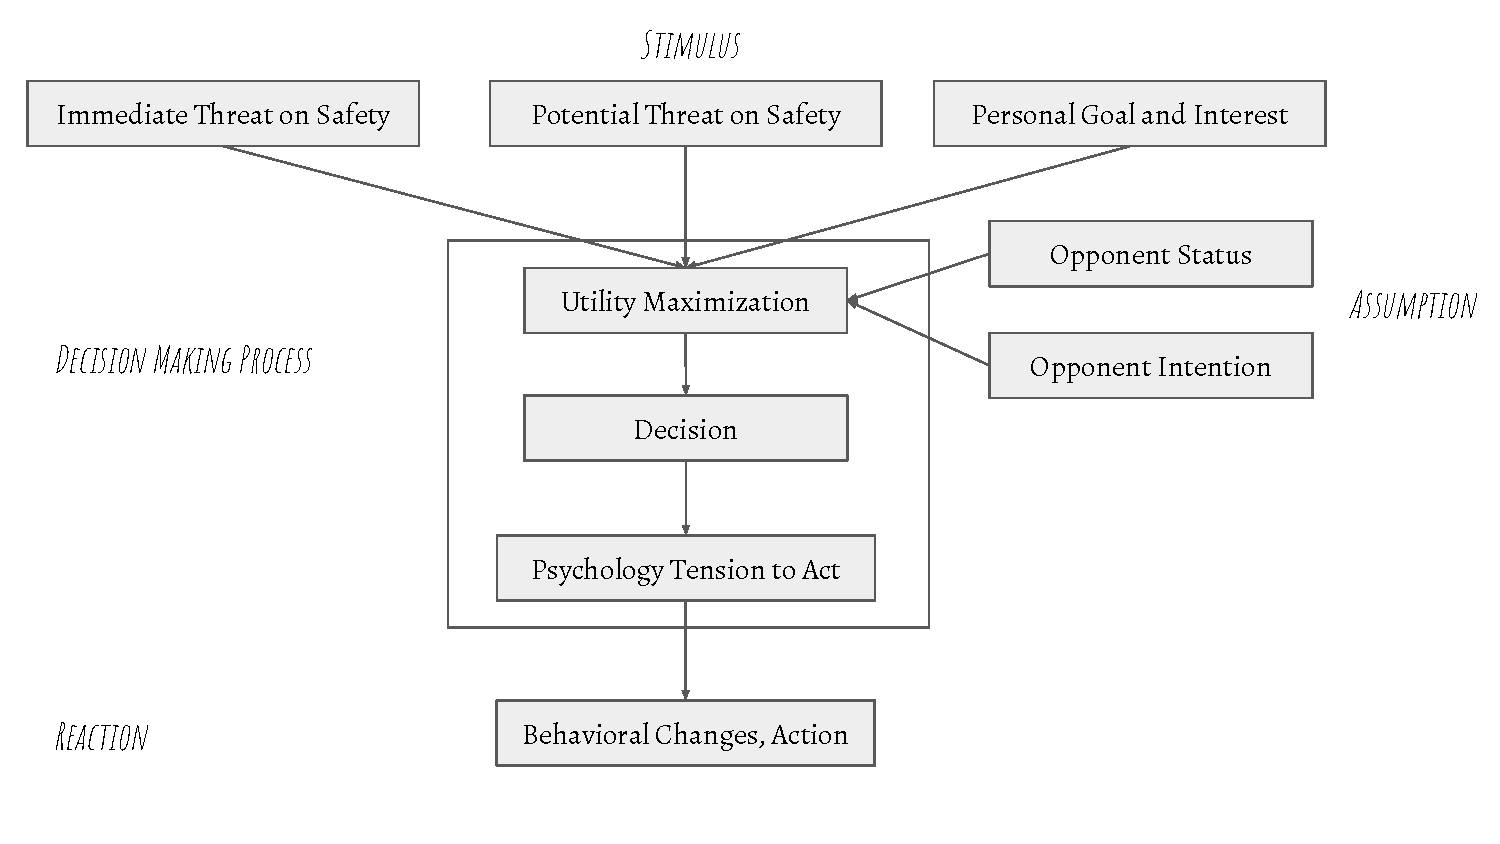
\includegraphics[width=1.05\columnwidth]{images/behavior_change.pdf}
  \hspace*{-2em}
  \vspace*{-1.5em}
  \end{center}
  \vspace{-0.05in}
  \caption{We propose this schematic illustration of human action model based 
    on the psychological process analysis on behavioral changes in ~\cite{helbing1995social}.
    Here, we further distinguish stimulus, and propose to include opponent 
    behavior into the decision making process.}
\vspace{-0.05in}
\label{fig:behavior}
\end{figure}
\vspace{-.3em}
\subsection{Human Decision Model considering Opponent Status and Intention Hypothesis}
We therefore propose to model people's decision making process during 
traversal considering both self stimulus and opponent agent hypothesis, as 
shown in Fig.~\ref{fig:behavior}. More specifically, we consider sources of 
stimulus based on levels of response time and frequency of variation. For 
example, goal and interest are usually fixed during the entire navigation 
process. Immediate instances such as unexpected turns of nearby agents cause 
direct threat and therefore stimulate responses quickly.

Our subject, the human traversal actions in crowds, are considered as potential 
threat due to possible future collision. It has certain response time after 
observing a confronting agent; it relies assumptions on 
opponent behaviors, to make the traversal decision that maximizes the person's 
own utility. 

Here, we list out the opponent assumptions on his status, defined as the 
abstract psychological state, and intention, defined as the potential 
action of interest. The opponent status can be estimated based on past 
observations, such as to distinguish if she is wondering in the hallway, or 
traveling towards a specific goal. The intention is what we care about the most at 
the end: is she going to cross me in the front or wait?

In human-robot interaction, the status goes beyond: is the person comfortable 
with the robot? Does she perceive the robot 
to be safe? As for intentions, we might further consider: is the person 
blocking/following the robot? 

In each case, we incorporate the opponent agent's influence into the decision 
making process. With that said, his action is taken into account while people 
consider their own actions. 
%%we hypothesis: people perceive the robot goal oriented, but the goal 
priority might be less important. They may perceive the robot as safe or 
unsafe, which largely affect their safety margin, response time, dynamic patterns.

\vspace{-.3em}
\subsection{Preliminary Results}
%heading variation suggests interactability
%different safety margins on traversal type decision
%psychology tension oh reaction time
%% however, more specifically: who have what interaction preferences? we don't 
%% know their intention, neither hypothesis of the robot. how can we achieve 
%% intent expressive motion in a human-friendly way?
Based on the above, we first study:
\begin{enumerate}
\item the opponent hypothesis in human-robot interaction, assuming 
  self-interested behaviors in a game setting: how people perceive the robot, 
  and decide their actions, in a goal-focused task?
\item the dynamic patterns during human traversal around a robot: how people 
  express their traversal intentions and what they expect on the robot's 
  response?
\end{enumerate}

We conduct experiments in an atrium with the robot following pre-assigned 
routes. We first show the participants how the robot runs the task, and then 
ask them to travel between four sets of waypoints that collision may happen in 
between. Each participant takes the experiment twice, with different values of 
safety margin ($0.3m$ and $1m$) that the robot keeps from the collision. Six 
people were invited in the test, with no prior experience to interact with the 
tested platform. We adopt a ROS people tracking package from ~\cite{leigh2015person}
on a Velodyne laser scanner. 

%Preliminary results are shown in Fig.~\ref{fig:pre_result}. 
Due to space constraint, graphical illustration of preliminary results are 
shown in the workshop session for discussion. 

We categorize people into four groups, based on their assumption of the 
robot's safety criteria (perceived opponent status), and their expectation on 
robot intention (opponent potential action), as being: cautious, comfortable, 
overly comfortable, or aggressive to the robot. Only people who assume the 
robot to be safe appear interactive to the robot during traversal. Others 
navigate straight to their goals with non-interactive routes, such as active 
passage with large safety margins. They also tend to react to potential 
collision much more in advance compared to (overly)comfortable people. 

Cautious people assume the robot to be unsafe and avoid the robot. Overly-comfortable 
people assume the robot to be safe and expect the robot to be only passively avoiding when 
humans take active action. Comfortable people assume the robot safe and change 
their actions when the robot's action is mismatched with their expectation. 
For example, they try to actively traverse the robot, but hold when they see 
the robot not immediately responding to their action. Aggressive people 
largely prefer to actively take way even with much deviation from the original path. 

The traversal maneuvers we observed fell into our proposed two homotopy 
classes, although interactive people may change their actions during the 
interaction. We propose to pursue this process as \textit{intention communication}, 
which converges when two agents reach consensus, and aim at enhancing the 
smoothness and efficiency of this process through intention-expressive robot 
motions.

%\begin{figure*}[tb]
%  \begin{center}
%  \hspace*{-6em}
%    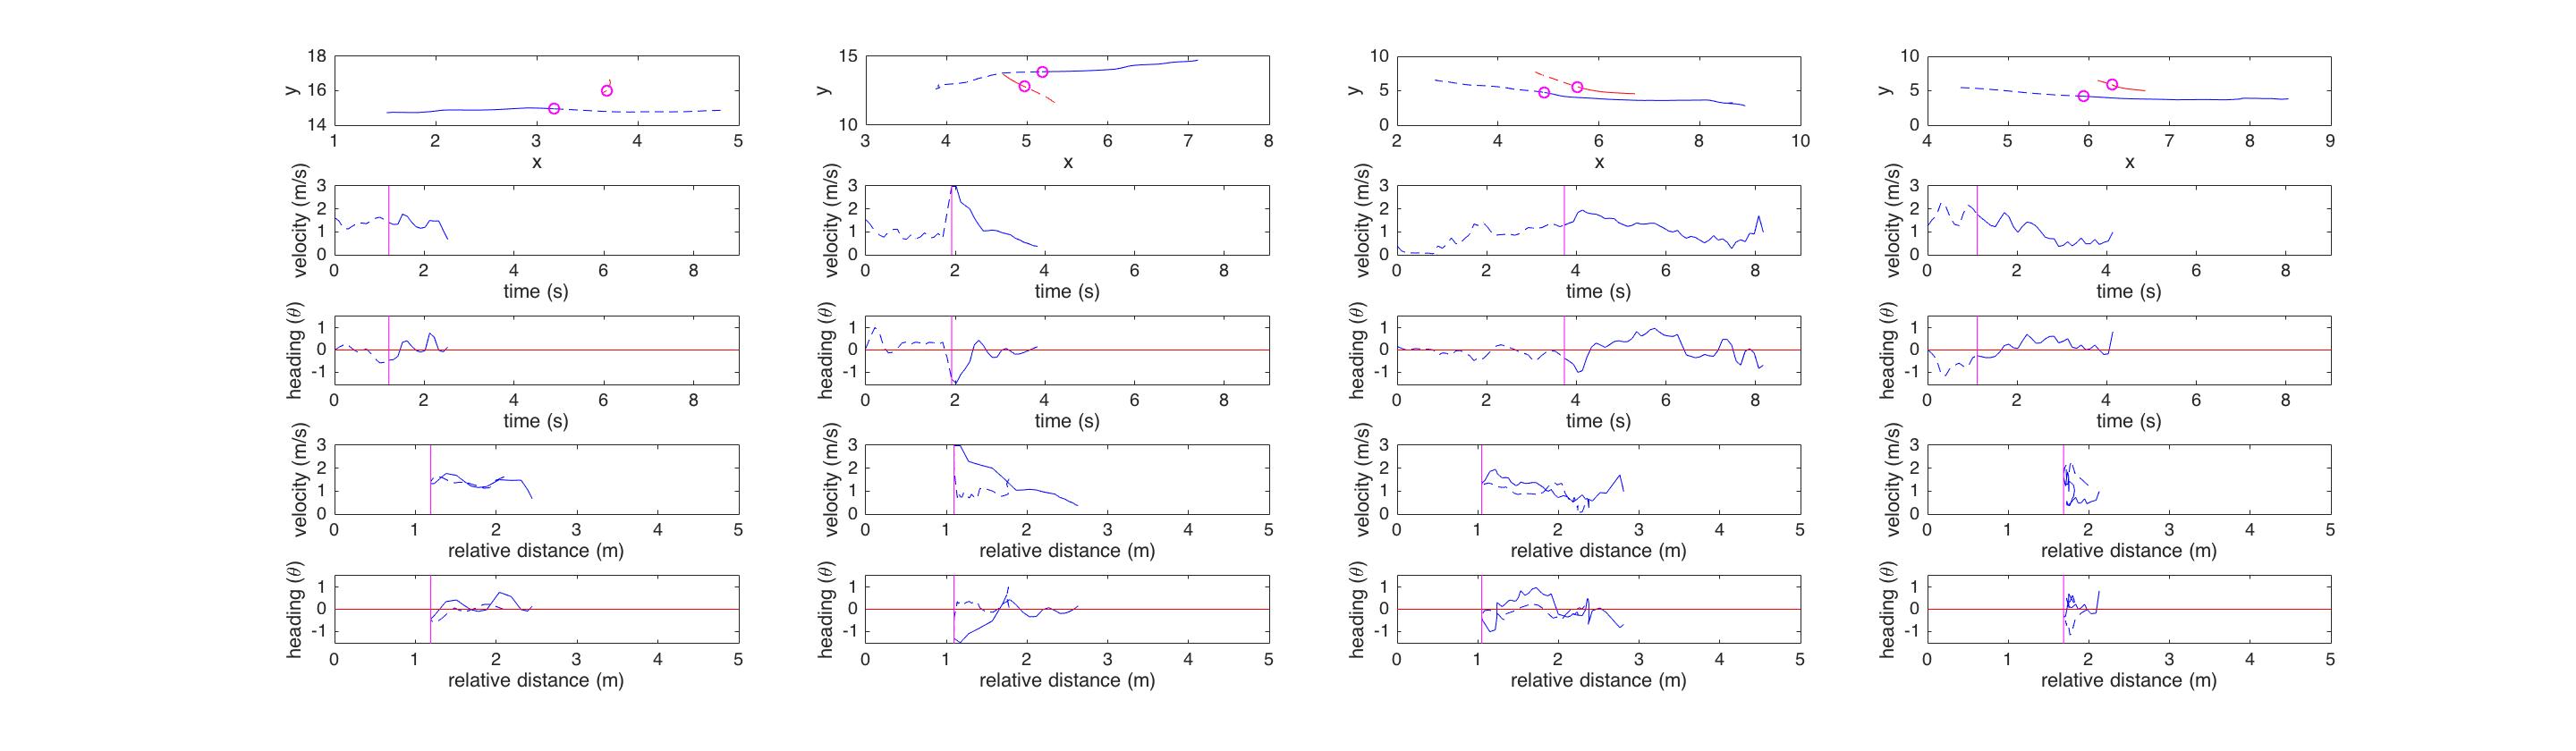
\includegraphics[width=1.2\textwidth]{images/dynamic_result2.png}
%  \hspace*{-1em}
%  \vspace*{-1.5em}
%  \end{center}
%  \vspace{-0.1in}
%  \caption{Preliminary results: from top to down, each row suggests: 
%    \textit{1.}close-distance interaction trajectories (red: robot, blue: 
%    pedestrian), \textit{2.}pedestrian velocity 
%    profile over time, \textit{3.}heading profile (velocity direction) over 
%    time, \textit{4.}velocity profile over the relative distance between two 
%    agents, \textit{5.}heading profile over the relative distance between two 
%    agents. Magenta circles/lines correspond to the closest interaction point. 
%    Dashed lines correspond to paths before closest interaction.}
%\label{fig:pre_result}
%\end{figure*}
\vspace{-.3em}
%\subsection{Mathematical Models}
%In situations where past observations are non-expressive to 
%distinguish human traversal types, safe and 
%intention-expressive maneuvers can evoke intention communication. Still, 
%without good estimate and prediction of human intentions, it is hard to 
%monitor intention communication quality. For this purpose, we propose to learn 
%two models to predict human intentions based on the above four pedestrian 
%types: before and after they interact with the robot.

%Before interaction, to understand the person's intention for the robot to 
%respond safely and efficiently, we model the pedestrian's action $a^h$ over 
%passive ($a^P$) or active action ($a^A$) by logistic regression,
%\begin{equation}
%p(a=a^P|\xi_t) \sim \frac{1}{1+e^{w^Tf(\xi_t)}},
%\end{equation}
%here, $f$ is a feature vector discriminating pedestrian types from past trajectories.

%Based on safety concerns and travel efficiency expectation, before the person 
%react to this potential collision, the robot can 
%decide to communicate intention $a^r= (a^P$ or $a^A$) through legible motion 
%realization ($\xi^A$ or $\xi^A$),
%\begin{equation}~\label{eq:transition}
%p(a^p=a^P|\xi_t, a^r) \sim \frac{1}{1+e^{w^Tf(\xi_t,a^r)}},
%\end{equation}
%and use this intention transition predictor for look-ahead planning.

%This process can only be iteratively learnt through robot real-world 
%deployment, considering people are also learning the maneuver of the robot.

%dynaimc transition (how they would react to robot legible motions)
%% definition of dynamics transition(our model applies to goal-oriented pople) 
%- whenever the person changes the maneuver to avoid the other agent (also, 
%when do they express intention, which they may express?)
% need to estimate collision location, response region, and safety margin

%% human-robot interaction intent hypothesis: different classes of people have 
%different social interactions, adaptive KF

%%intent expressive motion design - the leading agent




%% logistic regression on decision manifold
%Based on the continuous control input $u^o$ (here the robot acceleration), the 
%relative distance $d^{rel}$, and the adaptive safety margin $d^{saf}$ to 
%allow for unexpected behaviors of the robot, we model the pedestrian 
%decision making over passive ($a^p$) or active action ($a^a$) by logistic regression,
%\begin{equation}
%p(a=a^p|x,u^o) \sim \frac{1}{1+e^{w^Tf(x,u^o)}}, %%they should be of past trajectory?
%\end{equation}
%where $x$ is the overall system state, including the pedestrian and confronting agent, and $f(x,u)$ is a feature function, capturing the relative dynamics of the two agents.

%\section{Preliminary Results}
%Preliminary results have suggested the dependency of people's traversal preferences 
%on different regular walking patterns. For example, people who often traverse from 
%the front, have a higher regular walking pace. Since the traversal 
%behavior also depends on the robot's observed behaviors, we collect data under 
%different robot navigation policies. In this workshop, we intend to show the 
%robustness of the proposed pedestrian traversal decision predictor. We also 
%intend to show the learnt interactive dynamics during traversal, through phase 
%space analysis on velocity changes and positions. The resultant optimal 
%policy that maximizes both agents' efficiency is expected to act legibly 
%and responsively to the perceived human pedestrian traversal style. When the 
%prediction fails and the risk of collision goes up, it is quite likely that 
%the pedestrian is intentionally blocking the robot.
%%The decisions of pedestrians are modeled on both waypoint selections (mixture model on different ho%motopy classes, based on speed, relative speed, spacing, and safety margins) and speed pattern adapt%ation (adaptive slow down or speed up to avoid collision, based on the same features). 

\section{Future Work}
We look forward to seeing the transition dynamics described in Eq.~\ref{eq:transition} 
in real-world deployment, and use the pedestrian type features to better study 
the cost function formulation in Eq.~\ref{eq:social_cost}. After all, there is 
unresolved conflicts in human navigation models, such as the statement on 
visibility for planning~\cite{kruse2012legible} and dynamics modeling~\cite{helbing1995social}.

%% is it ok to cross from behind? From the social force, yes; from the social 
%% proximity on visibility - no. 


{\footnotesize
\bibliographystyle{plainnat}
\bibliography{reference}
}
\end{document}


